\chapter{Literature Review}\label{chapter-literature-review} 

The purpose of this chapter is to review the state-of-the-art literature of multi-modal attention. The first section describes attention in humans from both a psychological and a neurological point of view. We argue this will give the reader more intuition about attention in deep learning. The second part moves on to the different attention mechanisms in deep learning, in particular self-attention and crossmodal attention. 


%-----------------------------------
%	SECTION 
%-----------------------------------
\section{Attention in Humans}
The most profound effect of attention is its capacity to bring the attended stimuli into the forefront of our conscious experience while unattended stimuli fades into the background, increasing the processing efficiency at every stage of perception \citep{watzl}. A widely held assumption in the psychology literature is that the most fundamental function of attention is selection. At the level of single neurons, neuroscientists typically thought of attention in terms of selection between stimuli competing for the same neural receptive field \citep{neuro-level}. Daniel Kahneman, an authorithy in psychology and economy, investigated the way in which humans perform multi-tasking (i.e., solve a multi-modal problem). Kahneman claimed that attention was more than selection, that it could be viewed as a limited resource being shared among the different modes, but he could not generalize his findings to the intra-modal level\footnote{Intra-modal attention manifests itself only in a subset of the mode, whereas inter-modal attention is between modes.}. Moreover, the selection theory has been vigorously challenged in recent years by the amplification theory, where attention is an additional activity that interacts with built-in perceptual mechanisms by amplifying some of the input signals \citep{amplification}. Furthermore, the absolute intensity of amplification is not important, in contrary it is the relative intensity between the inputs that matters (\textit{the contrast effect}). Notice that the amplification theory generalizes the concept of capacity to the intra-modal level and neural level. Interestingly, we will see that the basic principles of attention mechanisms in deep learning has significant similarities with amplification.

Regarding multi-modal attention, three types can be distinguished: endogenous, exogenous and crossmodal attention \citep{crossmodal}. People orient their attention endogenously whenever they voluntarily choose to attend to something, such as when listening to a particular individual at a noisy cocktail party, or when concentrating on the texture of the object that they happen to be holding in their hands. By contrast, exogenous orienting occurs when a person’s attention is captured reflexively by the sudden onset of an unexpected event, such as when a mosquito suddenly lands on our arm. Lastly, crossmodal attention refers to the interaction of attention between two or more modes such as using visual clues (e.g. lip movements) to focus on the voice of a particular individual at a noisy cocktail party.


%-----------------------------------
%	SECTION 
%-----------------------------------
\section{Attention in Deep Learning}
Attention mechanisms in deep learning aim to highlight specific regions of the input space. The most common way to do this, is by multiplying the input by an attention mask, where the attention mask consist of normalized continous values between zero and one. Observe the similarity with the amplication theory described in the previous section. In self-attention \citep{bahdanau}, the attention mask is computed from the same mode on which it is applied. Conversely, for crossmodal attention mechanisms \citep{crossmodal-object-detection}, the attention mask is computed from multiple modes. 

Self-attention was first introduced in natural language processing (NLP) for machine translation tasks by \citep{bahdanau}. It helped the translation task by enabling the model to automatically search for parts of a source sentence that are relevant to predicting the next target work. With this approach, Bahdanau et al. achieved a translation performance comparable to the existing state-of-the-art phrase-based system on the task of English-French translation. Since then it has become a prominent tool in NLP but has also been used in a variety of other tasks such as image classification. \citep{self-capsule} uses self-attention to learn to suppress irrelevant regions in images and highlight salient features useful for the specific classification task. The authors in \citep{self-capsule} reduced the computation load and were able to compensate the absence of a deeper network by using the self-attention, without having a decreased classification performance. For a detailed review on this self-attention mechanisms, see \citep{attention-review}.

Turning now to crossmodal attention, \citep{looking-to-listen} presents an audio-visual model for isolating a single speech signal form a mixture of sounds such as other speakers and background noise (see Figure \ref{fig:looking-to-listen}). Crossmodal attention is used to focus on certain parts of the audio with respect to an image of the desired speaker. The authors showed superior results compared to state-of-the-art audio-only methods. Similar works \citep{cross-transformer, crossmodal-object-detection, crossmodal-video-caption} are using crossmodal attention and have attained impressive results. However, most research using crossmodal attention has tended to focus on obtaining better predictions rather than improving the robustness. A few exceptions are discussed below.
\begin{figure}[!ht]
\centering
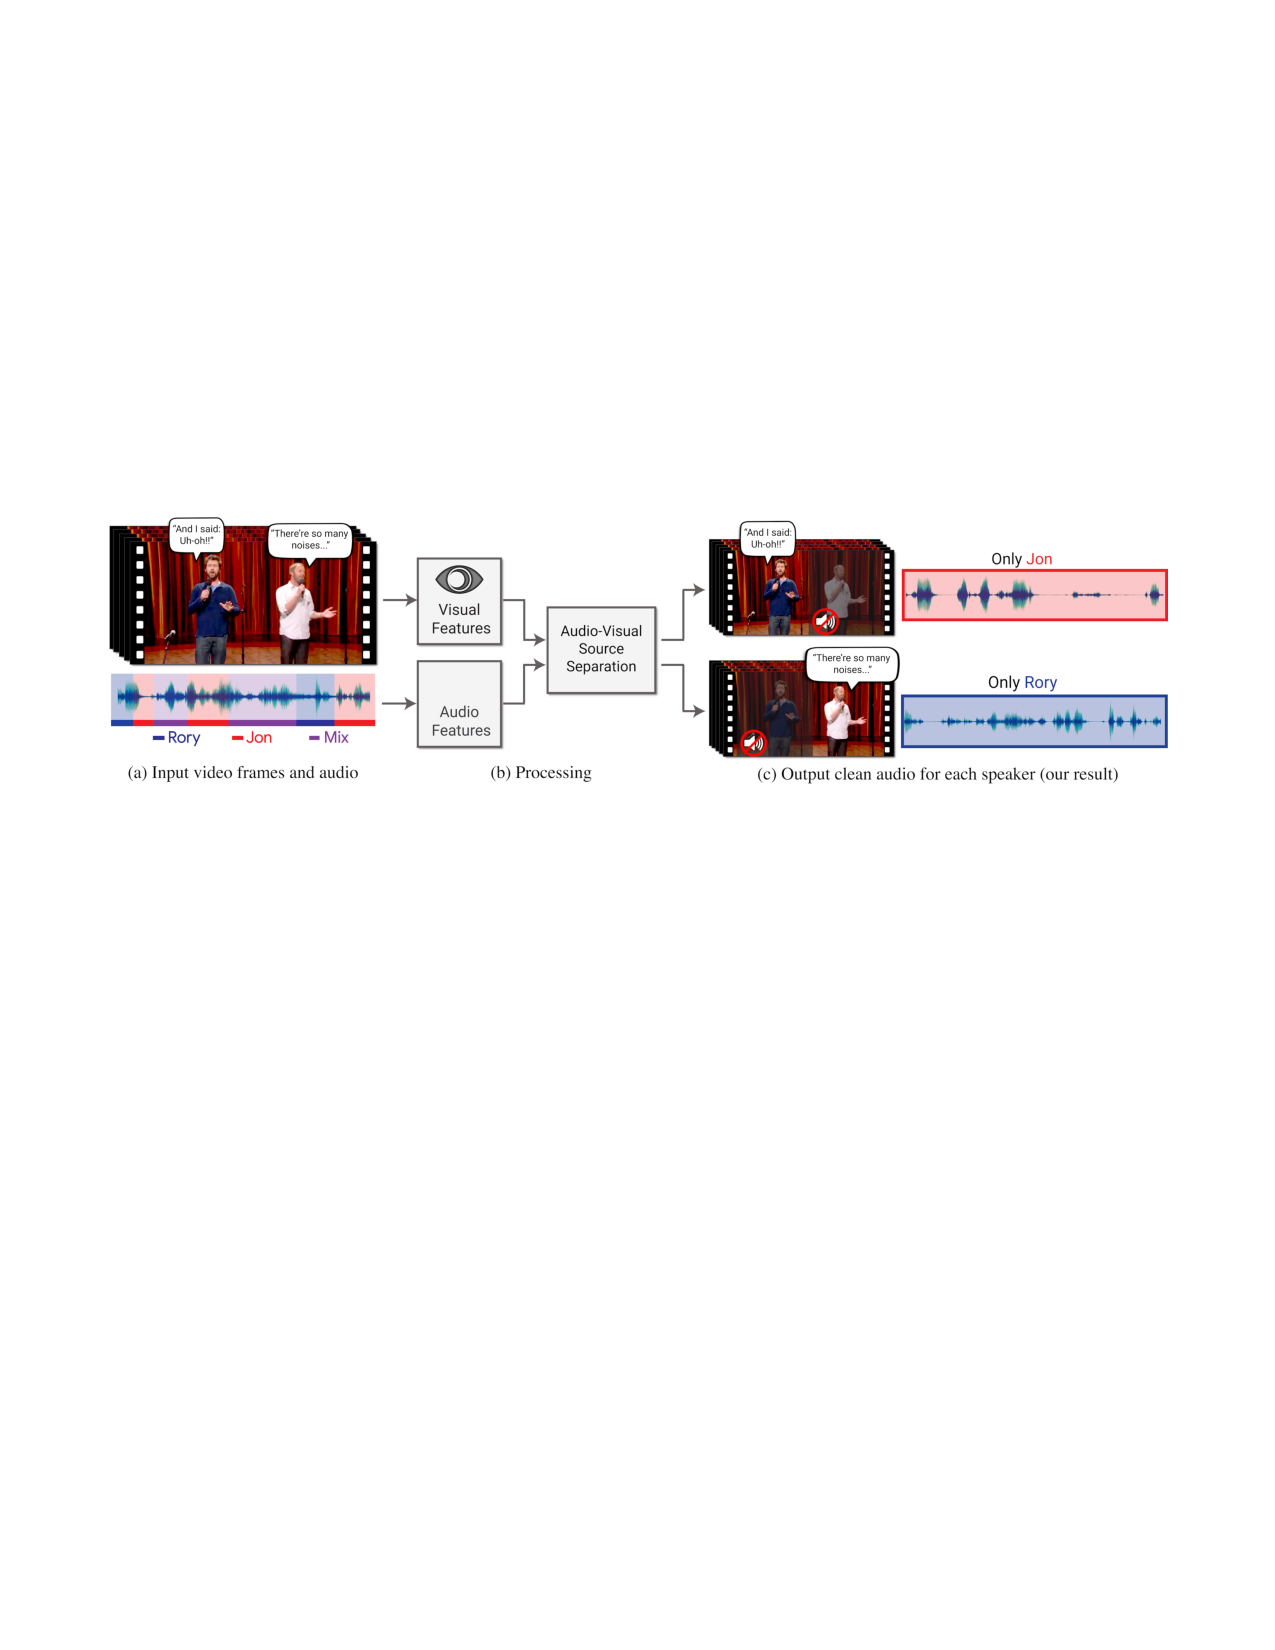
\includegraphics[scale=0.85]{figures/look-to-listen}
\caption[Looking to Listen framework]{The authors of \citep{looking-to-listen} present a model for isolating and enhancing the speech of desired speakers in a video. Their model was trained using thousands of hours of video segments from our new dataset, AVSpeech. \textit{Image from} \citep{looking-to-listen}}
\label{fig:looking-to-listen}
\end{figure}

A work investigating how multimodal fusion can help against failing modes is \citep{afouras}. Their model fuses audio and video to obtain better speech-to-text. Interestingly, Afouras et al. use a combination of self-attention mechanisms followed by a crossmodal attention layer. The model was tested on thousands of natural sentences of British television. Furthermore, they added babble noise with 0dB signal-to-noise ratio to the audio streams, where the babble noise samples are synthesized by mixing the signals of 20 different audio samples from the dataset. The audio-visual model achieved a 13.7\% word error rate (WER) on the dataset without noise, and a 33.5\% WER on the dataset with noise whereas the audio-only model only achieved 64.7\% WER. Despite obtaining great results, a major weakness with this experiment, however, is that their test set is corrupted in the exact same manner as their training set. In our experiments\footnote{See Section \ref{sec:generalization}} we will show that evaluating test data with the same noise as on the training data can significantly overestimate the robustness of the model. Additionally, the attention module in \citep{afouras} is presumably not able to detect and handle unseen samples. To summarize, the model was not tested against realistic failing modes situations.

The work that is most relevant to our proposed method is the attentive context proposed in \citep{audiovisual-attention}, which also incorporates attention on the inter-modal level to explicitly filter perturbations out (see Figure \ref{fig:noise-tolerant}). The model is evaluated on a face-verification task, receiving a \textbf{v}oice sound and a \textbf{f}ace image. The attention mask $[\alpha_v,\alpha_f]$ is computed via a linear function, $f_{\text{att}} = \mathbf{W}^T[\mathbf{e}_v, \mathbf{e}_f] + \mathbf{b}$, on the embeddings $\mathbf{e}_v$ and $\mathbf{e}_f$. Several defects of the attention function $f_{\text{att}}$ can be observed: 
\begin{enumerate}
\item The function is unlikely to be expressive enough to capture complicated dependencies between the modes, and to recognize out-of-distribution\footnote{Relative to the training data} data.
\item A design constraint of this attention function is that all extracted embeddings must be of the same size, which may be a significant constraint when combining modes from low and high-dimensional data.
\item Similarly to \citep{afouras}, the test set is corrupted in the same manner as the training set.
\end{enumerate}

\begin{figure}[!ht]
\centering
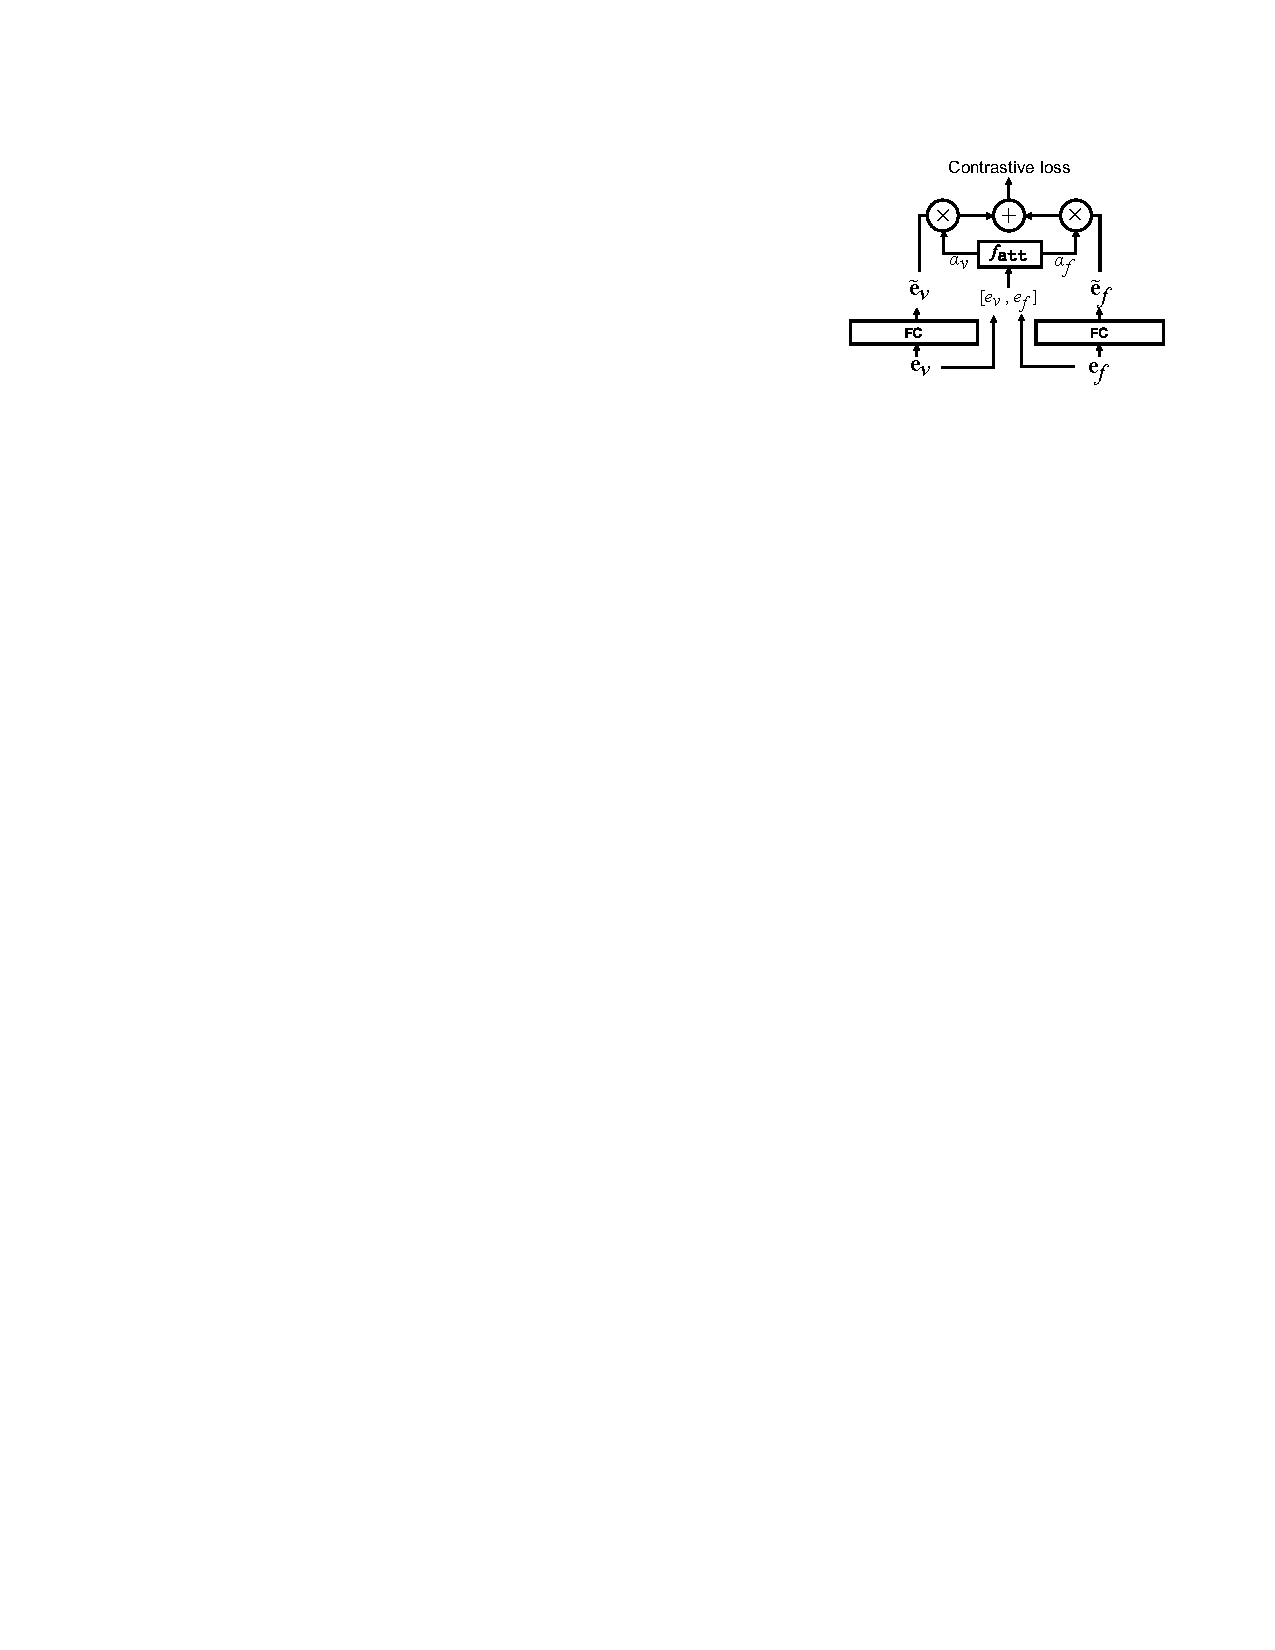
\includegraphics[scale=0.85]{figures/noise-tolerant}
\caption[Noise-tolerant fusion model]{Neural network based fusion approaches. $\mathbf{e}_v$ : speaker embedding, $\mathbf{e}_f$ : face embedding. FC denotes a fully connected layer. \textit{Image from} \citep{audiovisual-attention}}
\label{fig:noise-tolerant}
\end{figure}



